\chapter{Modelo do Fluxo de Atividades Atual do Produto Investigado}
\label{apdx:processo-antigo}

Este apêndice apresenta o processo de desenvolvimento já existente no produto sendo investigado, ilustrado nas Figuras \ref{fig:antigo-process-a} e \ref{fig:antigo-process-b}. O diagrama foi segmentado em duas partes para garantir a legibilidade de todas as fases, artefatos e atividades. As setas que conectam as figuras foram identificadas por letras em ordem alfabética, facilitando a compreensão do modelo como um todo.

\clearpage
\begin{landscape}
    \begin{figure}[p]
        \centering
        \caption{\textit{Modelo do Fluxo de Atividades Atual do Produto Investigado (Parte 1 de 2)}}
        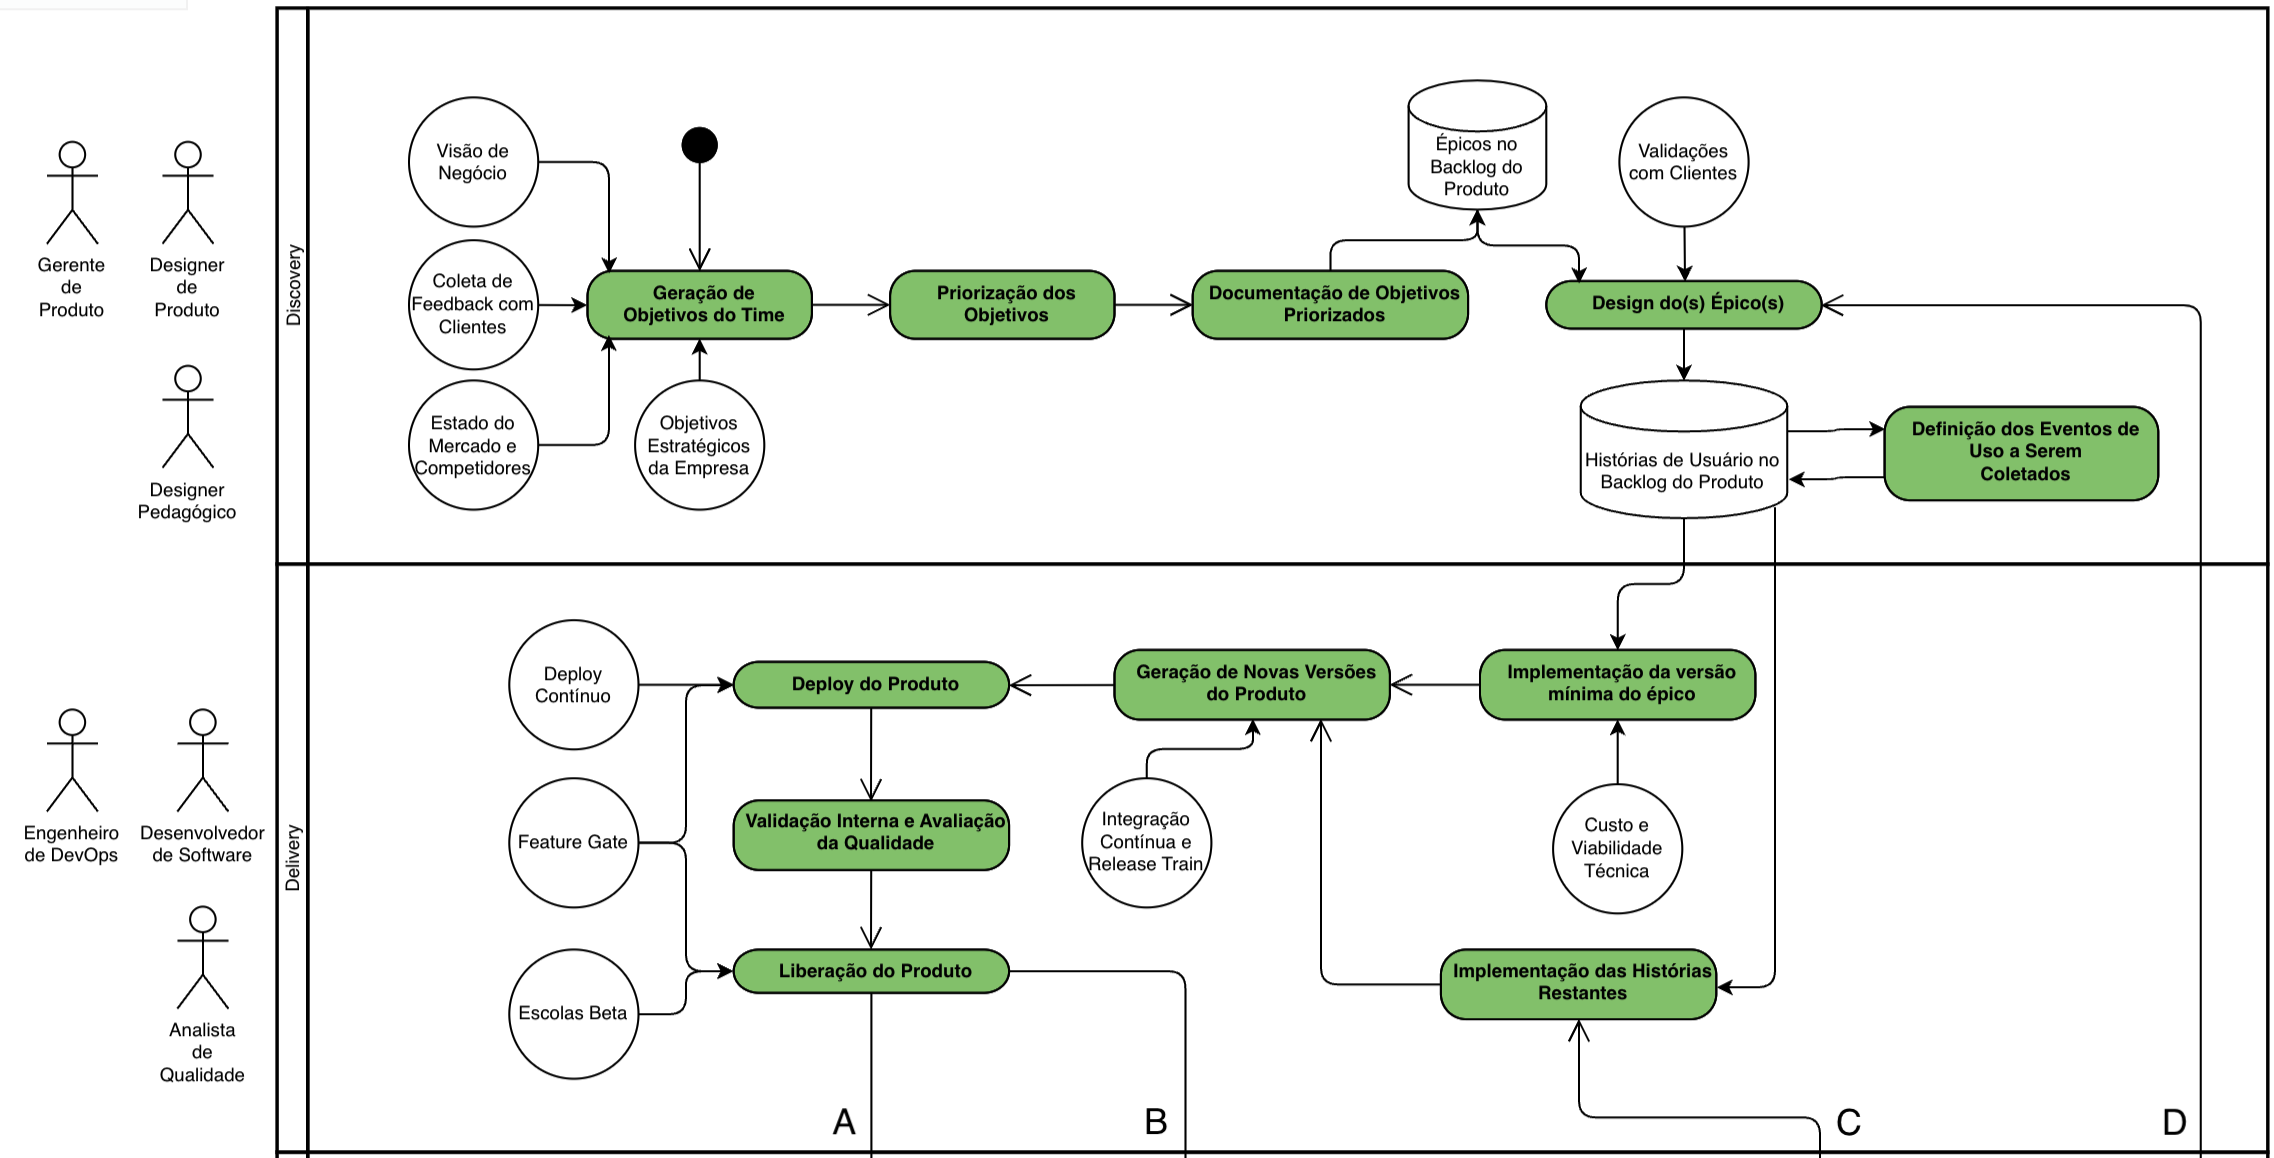
\includegraphics[width=1\linewidth]{figuras/processo_antigo_a.png}
        \text{Fonte: Autor}
        \label{fig:antigo-process-a}
    \end{figure}
\end{landscape}


\clearpage
\begin{landscape}
    \begin{figure}[p]
        \centering
        \caption{\textit{Modelo do Fluxo de Atividades Atual do Produto Investigado (Parte 2 de 2)}}
        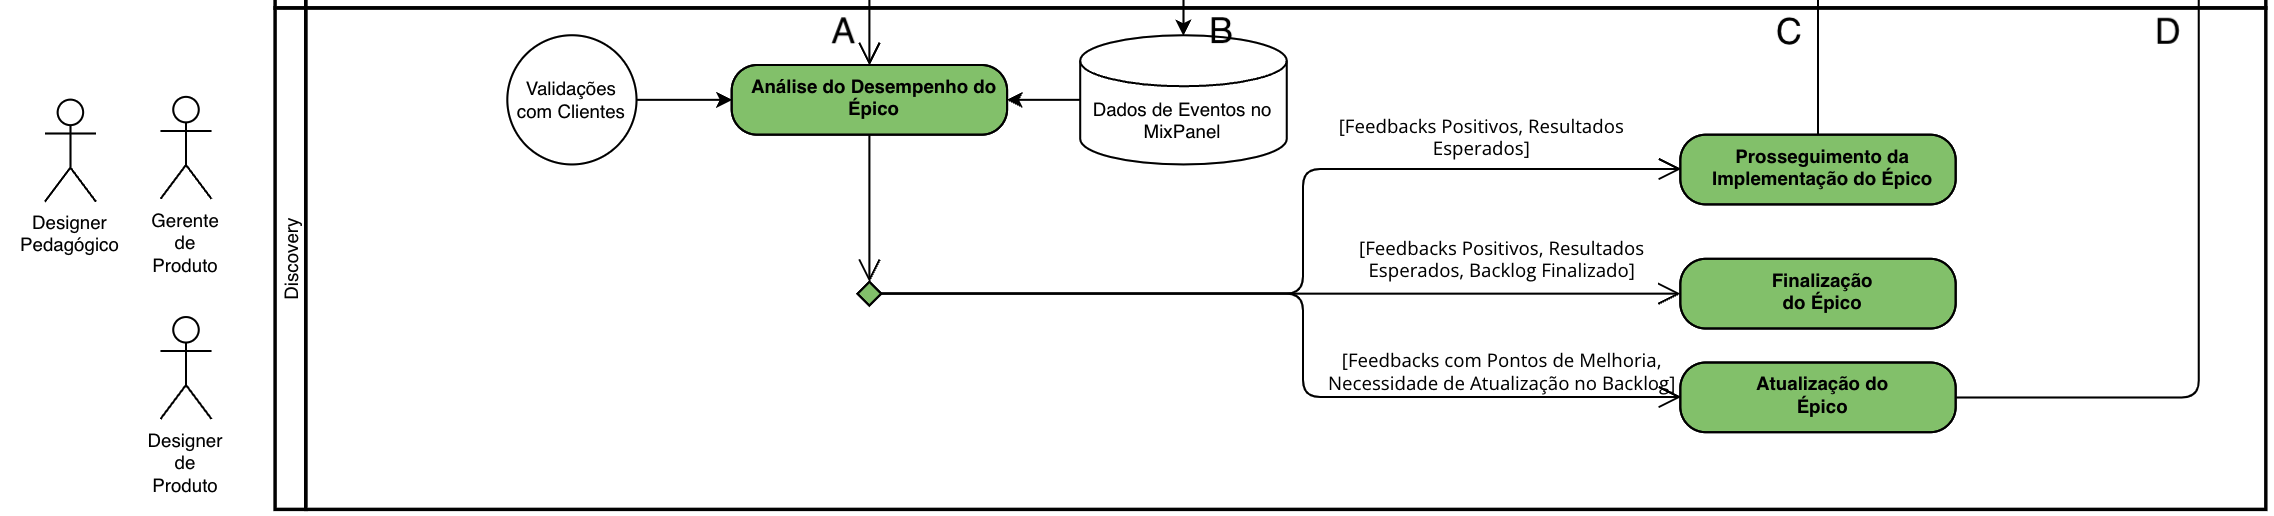
\includegraphics[width=1\linewidth]{figuras/processo_antigo_b.png}
        \text{Fonte: Autor}
        \label{fig:antigo-process-b}
    \end{figure}
\end{landscape}

